Our simulation consists of a set of agents that try to navigate a randomly
generated maze, these agents are meant to simulate robots in the real world. 
They communicate with a set agents that act as soft bots in web services. These
soft bots support the robots in accomplishing their task to rescue victims from
the maze. For communication between the agents we use the SPADE \footnote{https://pypi.python.org/pypi/SPADE} framework as our top layer.

\subsection{Simulation Model}
The simulation consists of two web services, two types of robots and a
central brain. The web services are a data store and a path planner. The data
store is used to store the map, while the path planner can be given a map, a
starting point and a target location. The robots can either be a search robot,
they can sense the environment; or they can be rescuers in which case they have
actuators and the capability to carry victims. The search bots explore the maze
with help from the central brain, while the rescue bots are sent into the maze
to collect the targets. The central brain is the link between all these
components. It also keeps track of the parts of the map that have been visited
and the areas of the map that have unexplored corridors. The central brain also
makes sure that the search bots are not all at the some location but explore
different parts of the map.

\subsubsection{Data Store agent}
This agent is responsible for storing the information that the search agents
gather while exploring the maze. The agent is a web service that acts like any
database but is also able to interact with agents instead of exposing an API.
This means that other agents can query and update the data that this agent
stores like any regular database.

\subsubsection{Path planner agent}
This is a web service that when given a map, a start position and a destination
position will plan the shortest path between these two positions. It plans the
paths by using the $A^*$ algorithm \cite{astar}. This agent is also able to
receive multiple destination positions and then responds with the shortest path
among those positions, this is also described in \autoref{alg:multidest}.

\begin{algorithm}
	\caption{Method to find the shortest available path between multiple
		destinations.}
	\label{alg:multidest}
	\begin{algorithmic}[1]
		\REQUIRE{Map $M$, begin position $s$, list of destinations $D$}
		\ENSURE{Path $p$}
		\STATE $p \gets A^*(M, s, d_1)$
		\FORALL{$d \in D$}
			\STATE $t \gets A^*(M, s, d)$
			\IF{$\|t\| < \|p\|$}
				\STATE $p \gets t$
			\ENDIF
		\ENDFOR
	\end{algorithmic}
\end{algorithm}

\subsubsection{Search robot agents}
The search bots are robots that are simple platforms with some sensors. They
can be thought of as the eyes of the system, these agents are also able to move
around the maze quickly. This makes them ideal for searching through buildings.
They travel through the maze along the straight corridors until they reach a
fork in the maze. Then they call upon the central brain to give them a new
target to travel to and explore. If they get stuck in a dead end they will
request a new search location from the central brain. They will then ask the
path planning service to return a route to get to the new search location.

\subsubsection{Rescue robot agents}
Victims that have been found in the maze by the search robots need to be
rescued in some fashion but the search robots are not equipped for this. This
is where the rescue robots come in, they also represent physical robots and
they are the hands of the system. Rescue robots aren't equipped with sensors to
map out the maze. Instead they have actuators that allow them to carry victims
around. These agents are send a target location by the central brain and then
they move to that location, pick up the victim at the target and then move to
the exit of the maze to rescue them.

\subsubsection{Supervisor agent}
The Supervisor is the central part of the system that makes sure that all
the components work together. It manages most of the resources and it keeps
track of where robots are. It also directs all the search robots and to make
sure that they don't all try to explore the same area. It also directs the
rescue bots to the victims and makes sure that only one rescue bot tries to
rescue each victim.

\subsubsection{Interaction}
Every time a search agent uncovers a new location, it will send a message to
the data store so it can be updated with the additional data. This information
can later be retrieved.

When a search bot gets stuck, it reports its current location to the central
brain . The central brain then requests the current map. Then it sends the
map, the location of the stuck searcher and a position that has not been
visited yet to the path planner. The planner will return a path if it is
possible. The central brain then sends this path to the searcher so it can
resume exploring.

\subsection{Experimental design}
The central brain is an important link in our system, and we would want it to
be as robust as possible. Therefore we would want to know whether the
system performs better if the central brain is one monolithic object or if
there is division of labour between the agents. For this we implemented
multiple structures for the central brain, one where the brain is a central
director orchestrating all agents and one where all agents are
communicating with each other. 

To test this, we had different configurations of search agents and rescue
agents that we placed into a maze of 8 by 8 with 5 targets. The agents had
to explore the whole maze and rescue all the targets. The time they needed
to do this was measured. This, included the startup time and the shutdown
time for the agents. The time needed to rescue all the targets and discover
the full maze (rescue time) is our indication of performance. The system
will need to explore the full maze to make sure that all targets are found.

We ran the simulation once with 1 search and 1 rescue agent as a baseline.
We do not expect to see a difference in the results for this configuration,
since the mothership should be able to handle one agent as well as the
distributed supervisor. We also ran the experiment with 3 searchers and 3
rescuers. And to also see if the number of searcher agents with influence
the result, we also ran the simulation with 3 rescue agents and 6 search
agents. 

The simulation was run several times per configuration. All the simulations
were run on the same machine, to make sure the different rescue times could
be compared. 

\begin{figure}[h]
	\centering
		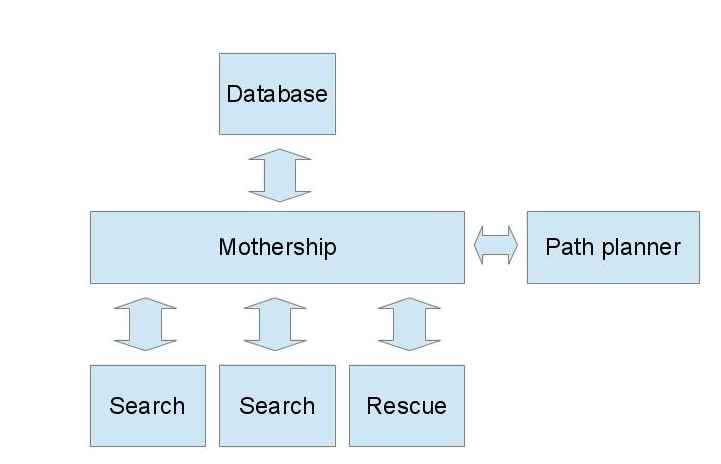
\includegraphics[width=6cm]{mothership}
	\caption{Mothership overview}
	\label{fig:mothership}
\end{figure}

\begin{figure}[h]
	\centering
		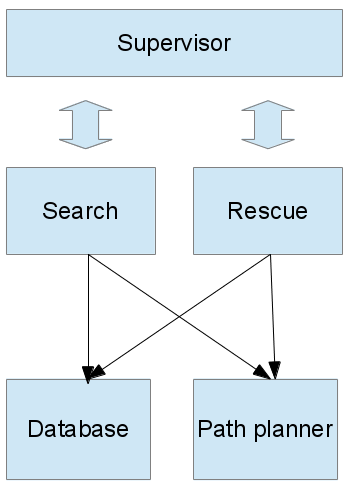
\includegraphics[width=6cm]{supervisor}
	\caption{Supervisor overview}
	\label{fig:supervisor}
\end{figure}
